\documentclass[
%% TIKZ_CLASSOPTION %%
tikz
]{standalone}
\usepackage{amsmath}
\usetikzlibrary{matrix}
%% EXTRA_TIKZ_PREAMBLE_CODE %%
\begin{document}
%% TIKZ_CODE %%
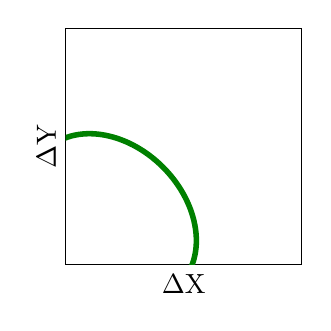
\begin{tikzpicture}[scale=3]
   \draw (0,1) -- node[rotate=90,above] {$\Delta$Y} (0,0)
      -- node[below] {$\Delta$X}(1,0) -- (1,1)  -- (0,1);
   \begin{scope}
     \clip(0,0) rectangle (1,1);
     \draw[color=green!50!black, line width=2] (.2,.2) circle[x radius=.3, y radius=.4, rotate=45];
   \end{scope}
\end{tikzpicture}
\end{document}
